\documentclass[
11pt, % The default document font size, options: 10pt, 11pt, 12pt
%codirector, % Uncomment to add a codirector to the title page
]{Clases/charter} 


\usepackage{eurosym}

% El títulos de la memoria, se usa en la carátula y se puede usar el cualquier lugar del documento con el comando \ttitle
\titulo{Aplicaciones de modelos de lenguaje de Inteligencia Artificial (LLM) en la ambientación narrativa} 

% Nombre del posgrado, se usa en la carátula y se puede usar el cualquier lugar del documento con el comando \degreename
%\posgrado{Carrera de Especialización en Sistemas Embebidos} 
%\posgrado{Carrera de Especialización en Internet de las Cosas} 
\posgrado{Carrera de Especialización en Inteligencia Artificial}
%\posgrado{Maestría en Sistemas Embebidos} 
%\posgrado{Maestría en Internet de las cosas}

% Tu nombre, se puede usar el cualquier lugar del documento con el comando \authorname
\autor{Ing. Mario Gómez Alonso} 

% El nombre del director y co-director, se puede usar el cualquier lugar del documento con el comando \supname y \cosupname y \pertesupname y \pertecosupname
\director{Por ser definido}
\pertenenciaDirector{Por ser definida} 
% FIXME:NO IMPLEMENTADO EL CODIRECTOR ni su pertenencia
\codirector{John Doe} % para que aparezca en la portada se debe descomentar la opción codirector en el documentclass
\pertenenciaCoDirector{FIUBA}

% Nombre del cliente, quien va a aprobar los resultados del proyecto, se puede usar con el comando \clientename y \empclientename
\cliente{Ing. Hans Manuel Grenner Noguerón}
\empresaCliente{Critical Match}

% Nombre y pertenencia de los jurados, se pueden usar el cualquier lugar del documento con el comando \jurunoname, \jurdosname y \jurtresname y \perteunoname, \pertedosname y \pertetresname.
\juradoUno{Nombre y Apellido (1)}
\pertenenciaJurUno{pertenencia (1)} 
\juradoDos{Nombre y Apellido (2)}
\pertenenciaJurDos{pertenencia (2)}
\juradoTres{Nombre y Apellido (3)}
\pertenenciaJurTres{pertenencia (3)}
 
\fechaINICIO{17 de octubre de 2023}		%Fecha de inicio de la cursada de GdP \fechaInicioName
\fechaFINALPlan{5 de diciembre de 2023} 	%Fecha de final de cursada de GdP
\fechaFINALTrabajo{Por ser definido}	%Fecha de defensa pública del trabajo final


\begin{document}

\maketitle
\thispagestyle{empty}
\pagebreak


\thispagestyle{empty}
{\setlength{\parskip}{0pt}
	\tableofcontents{}
}
\pagebreak


\section*{Registros de cambios}
\label{sec:registro}


\begin{table}[ht]
	\label{tab:registro}
	\centering
	\begin{tabularx}{\linewidth}{@{}|c|X|c|@{}}
		\hline
		\rowcolor[HTML]{C0C0C0}
		Revisión & \multicolumn{1}{c|}{\cellcolor[HTML]{C0C0C0}Detalles de los cambios realizados}            & Fecha                   \\ \hline
		0        & Creación del documento                                                                     & \fechaInicioName        \\ \hline
		1        & Se completa hasta el punto 5 inclusive                                                     & 31 de octubre de 2023   \\ \hline
		2        & Aplicadas correcciones sobre la versión anterior y se completa hasta el punto 9 inclusive  & 7 de noviembre de 2023  \\ \hline
		3        & Aplicadas correcciones sobre la versión anterior y se completa hasta el punto 12 inclusive & 15 de noviembre de 2023 \\ \hline
		4        & Aplicadas correcciones sobre la versión anterior y se completa el plan en su totalidad     & 23 de noviembre de 2023 \\ \hline
	\end{tabularx}
\end{table}

\pagebreak



\section*{Acta de constitución del proyecto}
\label{sec:acta}

\begin{flushright}
	Buenos Aires, \fechaInicioName
\end{flushright}

\vspace{2cm}
Por medio de la presente se acuerda con el \authorname\hspace{1px} que su Trabajo Final de la \degreename\hspace{1px} se titulará ``\ttitle'',
consistirá esencialmente en la implementación de un servidor web que aloje una Inteligencia Artificial de tipo LLM que genere contenido narrativo a través de servicios REST,
y tendrá un presupuesto preliminar estimado de 695 h (de las cuales 80h son opcionales) de trabajo y \$5.396.529,2 (del cual \$551.020,8 es el coste de las horas opcionales),
con fecha de inicio \fechaInicioName\hspace{1px} y fecha de presentación pública \fechaFinalName.

Se adjunta a esta acta la planificación inicial.

\vfill

% Esta parte se construye sola con la información que hayan cargado en el preámbulo del documento y no debe modificarla
\begin{table}[ht]
	\centering
	\begin{tabular}{ccc}
		\begin{tabular}[c]{@{}c@{}}Dr. Ing. Ariel Lutenberg \\ Director posgrado FIUBA\end{tabular} & \hspace{2cm} & \begin{tabular}[c]{@{}c@{}}\clientename \\ \empclientename \end{tabular} \vspace{2.5cm} \\
		\multicolumn{3}{c}{\begin{tabular}[c]{@{}c@{}} \supname \\ Director del Trabajo Final\end{tabular}} \vspace{2.5cm}                                                                                   \\
		%\begin{tabular}[c]{@{}c@{}}\jurunoname \\ Jurado del Trabajo Final\end{tabular}     &  & \begin{tabular}[c]{@{}c@{}}\jurdosname\\ Jurado del Trabajo Final\end{tabular}  \vspace{2.5cm}  \\
		%\multicolumn{3}{c}{\begin{tabular}[c]{@{}c@{}} \jurtresname\\ Jurado del Trabajo Final\end{tabular}} \vspace{.5cm}                                                                     
	\end{tabular}
\end{table}


\section{1. Descripción técnica-conceptual del proyecto a realizar}
\label{sec:descripcion}
El proyecto a realizar se enfoca en ampliar las herramientas que ofrece el producto Critical Match,
creado por la empresa con el mismo nombre y el cual consta actualmente de una aplicación para Android y iOS.
Concretamente, se trata de un proyecto personal donde la empresa Critical Match será el cliente.

La principal función de la App es permitir a sus usuarios la creación o búsqueda de salas de juego,
también conocidas como mesas, donde pueden unirse a otros jugadores para organizar partidas de rol,
ya sea en línea o de forma presencial.
Las mesas ofrecen un marco narrativo para que los usuarios seleccionen la que más se ajuste a sus preferencias.

Es en este punto donde se desea ampliar la funcionalidad mediante la incorporación de servicios de Inteligencia artificial para generar,
a partir de un contexto narrativo, una amplia gama de elementos adicionales.
Por ejemplo, personajes no jugables que se integren coherentemente en el mundo propuesto,
eventos que enriquezcan la trama y objetos, entre otros.

El estado del arte no está suficientemente avanzado en este aspecto.
Las soluciones de Inteligencia Artificial como ChatGPT, aunque competentes,
no suelen alcanzar los criterios de profundidad y precisión más exigentes,
lo que no siempre satisface las expectativas de los jugadores de rol.

Por otro lado, existen sitios web como WorldAnvil que ofrece a sus usuarios la posibilidad de crear y gestionar sus mundos de ficción,
donde la compleción de todas y cada una de las categorías y elementos del mundo recae exclusivamente en el propio usuario.
Es habitual que los moderadores de las partidas utilicen estas herramientas para compilar todo el contexto narrativo en un único lugar.
La empresa Critical Match quiere incorporar esta funcionalidad en su aplicación en un futuro cercano.

El objetivo principal del proyecto es crear una Inteligencia Artificial capaz de dar mejores resultados que otros motores como ChatGPT en un contexto de generación de texto de ambientación narrativa.
Esto implica desarrollar un sistema de IA altamente especializado y entrenado específicamente para la generación de contenido narrativo relacionado con partidas de rol, ofreciendo una profundidad y precisión que supere las limitaciones de las soluciones generales.

Adicinalmente, se busca dividir esta funcionalidad en varios servicios REST
(\textit{Representational State Transfer Protocol} o Protocolo de Transferencia de Estado Representacional)
para que la aplicación de Critical Match pueda acceder a las funciones de generación de contenido de forma remota.
Esto permitirá a los organizadores de las mesas de rol acceder a las capacidades de la IA,
integrando de manera transparente la ambientación narrativa generada en sus partidas y facilitando la creación de un mundo de ficción coherente y atractivo para los jugadores.

Se prevé que la Inteligencia Artificial se aloje en un servidor que sea accesible a través de peticiones REST (figura \ref{fig:diagBloques}).
Esto implica que el sistema de IA estará desplegado en un servidor remoto que estará constantemente en línea y disponible por el protocolo previamente mencionado.

\begin{figure}[htpb]
	\centering
	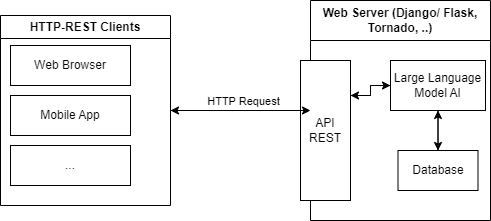
\includegraphics[scale=0.75]{./Figuras/diagBloques.png}
	\caption{Diagrama en bloques del sistema.}
	\label{fig:diagBloques}
\end{figure}
\vspace{25px}

En resumen, la propuesta de valor de este proyecto es la implementación de una serie de servicios REST que serán accedidos por aplicaciones externas,
principalmente Critical Match. Estos servicios permitirán la generación de elementos de ambientación narrativa, basados en el contexto del mundo proporcionado por los usuarios.

Esta iniciativa supone una evolución natural de la App Critical Match.
Actualmente el producto dispone de la funcionalidad de crear mesas y reunir jugadores y esta propuesta añade valor al facilitar a los organizadores de las partidas la creación de contenido atractivo para todos los participantes.

Además, este proyecto podría encajar en otros ámbitos que actualmente están enfocados en el “World Building” al proporcionar a creadores de mundos y escritores herramientas para expandir sus ideas.

Este proyecto a su vez es escalable y permite añadir nuevos servicios con el paso del tiempo.
Esto podría llevar en un futuro a la posibilidad de ofrecer un director de juego automatizado por Inteligencia Artificial que sea de interpretar las reglas y acciones de sus jugadores,
llevando a cabo partidas de rol de manera autónoma.


\section{2. Identificación y análisis de los interesados}
\label{sec:interesados}

\begin{table}[ht]
	%\caption{Identificación de los interesados}
	%\label{tab:interesados}
	\begin{tabularx}{\linewidth}{@{}|l|X|X|l|@{}}
		\hline
		\rowcolor[HTML]{C0C0C0}
		Rol         & Nombre y Apellido & Organización    & Puesto                        \\ \hline
		Cliente     & \clientename      & \empclientename & co-fundador de Critical Match \\ \hline
		Responsable & \authorname       & FIUBA           & Alumno                        \\ \hline
		Director    & \supname          & \pertesupname   & Director Trabajo final        \\ \hline
	\end{tabularx}
\end{table}

De esta lista podemos destacar:
\begin{itemize}
	\item Cliente y usuario final: \clientename.
	      Aporta contexto necesario sobre la App Critical Match y es el interesado de las herramientas que se desarrollarán en el proyecto.
	      Punto de contacto entre el responsable del proyecto y el equipo de Critical Match.
\end{itemize}

\section{3. Propósito del proyecto}
\label{sec:proposito}
El propósito del proyecto es el desarrollo de un servidor web que aloje una Inteligencia Artificial de tipo LLM.
Esta IA será entrenada para la generación de contexto y contenido narrativo.
El servidor podrá recibir peticiones a través del protocolo API REST,
donde se alimentará a la IA con un contexto narrativo.
El servidor responderá las peticiones con la salida aportada por el modelo
dependiendo de la entrada de texto y el tipo de servicio solicitado.


\section{4. Alcance del proyecto}
\label{sec:alcance}

El alcance del proyecto incluye lo siguiente:
\begin{itemize}
	\item Desarrollo de un servidor web.
	\item Entrenamiento de una Inteligencia Artificial de tipo LMM.
	\item Análisis y tratamiento de los datos utilizados para el entrenamiento de la IA.
	\item La integración de un conjunto esencial de servicios REST.
	\item Servicios adicionales, si entran dentro de las horas estimadas del proyecto.
\end{itemize}

El alcance del proyecto no incluye:
\begin{itemize}
	\item Página web.
	\item Securización del servidor web ni de ninguno de sus servicios REST.
	\item Rendimiento de los servicios que garanticen tiempos de respuesta cercanos a tiempo real.
\end{itemize}

En resumen, el proyecto consistirá de un prototipo que aporte funcionalidad en un tiempo de respuesta razonable,
pero es posible que no se ajuste a los requerimientos de un sistema puesto en producción.
Con esto aclarado, la intención siempre será desarrollar el proyecto aportando el mayor rendimiento posible.


\section{5. Supuestos del proyecto}
\label{sec:supuestos}
Para el desarrollo del presente proyecto se supone que:

\begin{itemize}
	\item No se desarrollará la Inteligencia Artificial desde cero, si no que se utilizará una pre-entrenada y de código abierto.
	      Partiendo de esa base, se hara un proceso de \textit{fine-tuning} para especializar el modelo en los servicios de generación de contenido narrativo.
	\item No se dispone de un set de datos por parte del cliente.
	      Se analizarán sets de datos con licencia abierta en la red y se emplearán aquellos que se ajusten al proyecto.
	\item Comunicación fluida con el Equipo de Critical Match para seguimiento del proyecto y aportación de ideas.
	\item El proyecto se realizará con una máquina cuyas especificaciones permitan tanto el desarrollo del código como su ejecución, además del proceso de \textit{fine-tuning} de la Inteligencia artificial.
	\item La disponibilidad para realizar las tareas del proyecto, las cuales se describirán más adelante, será de entre 20 y 30 horas semanales.
\end{itemize}


\section{6. Requerimientos}
\label{sec:requerimientos}
\begin{enumerate}
	\item Requerimientos del servidor:
	      \begin{enumerate}
		      \item El servidor debe alojar y administrar la información relativa al \textit{dataset} y la configuración del modelo LLM.
		      \item El servidor debe contar con los procesos necesarios para entrenar la Inteligencia Artificial.
		      \item Al ser desplegado, el servidor deberá iniciar el módulo LLM y utilizarlo en el procesamiento de peticiones entrantes.
		      \item El servidor debe dar acceso a clientes externos a través del protocolo API REST.
		      \item Los servicios REST deben aceptar entrada de texto en varios formatos: pdf, txt, word o texto plano en el cuerpo de la petición.
		      \item Los servicios REST devolverán la respuesta en formato simple HTML para su cómoda visualización en un navegador.
		      \item El prototipo del servidor debe de tener una disponibilidad del 100\% durante las pruebas y aceptar la carga de trabajo de peticiones individuales.
		            Opcionalmente, sería deseable que maneje el mayor número de peticiones simultáneas posible.
	      \end{enumerate}
	\item Requerimientos del módulo LLM:
	      \begin{enumerate}
		      \item El módulo LLM debe aceptar entrada de texto y generar texto como salida.
		      \item El módulo LLM, si el texto de entrada es legible, debe aportar una respuesta con un detalle y profundidad razonables,
		            además de ser coherente con las instrucciones recibidas.
		      \item El módulo debe disponer de múltiples métodos para los cuales, dada la misma entrada de texto, devolverá información enfocada en un aspecto concreto de la narrativa.
		            Por ejemplo, un método centrado en la generación de personajes, otro en la descripción de localizaciones, un tercero de eventos y así sucesivamente.
		      \item El tiempo de respuesta del módulo LLM debe estar, teniendo en cuenta el \textit{hardware} con el que se dispone, la extensión del texto de entrada y que no se garantiza un rendimiento cercano a tiempo real,
		            en un rango de tiempo razonable para un servicio REST (no más de 5 minutos).
	      \end{enumerate}
	\item Requerimiento de testing:
	      \begin{enumerate}
		      \item El proyecto contará con test automáticos que probarán el correcto funcionamiento de los módulos no relacionados con el modelo LLM.
		      \item El cliente podrá validar los test automáticos a través de un análisis del código.
		      \item Se validará con el cliente tanto el módulo LLM como el servidor.
	      \end{enumerate}
	\item Requerimientos de documentación:
	      \begin{enumerate}
		      \item Se entregará un documento de administrador que explicará brevemente el sistema, qué comandos de ejecución tiene y los requisitos \textit{hardware} necesarios para su correcto funcionamiento.
		            Además, contará con una descripción de todos los servicios REST disponibles en el servidor y un ejemplo de cómo acceder a ellos.
		            Este documento también recopilará las instrucciones de despliegue con la creación del entorno virtual, instalación de librerías y el entrenamiento del modelo, entre otros.
		      \item Se entregará un documento con un breve análisis de los resultados del módulo LLM que se hayan expuesto al cliente durante las reuniones de seguimiento.
	      \end{enumerate}
	\item Requerimientos legales:
	      \begin{enumerate}
		      \item Cualquier información del cliente que se utilice en el desarrollo del proyecto estará amparada por derechos de privacidad y propiedad intelectual.
		      \item El set de datos utilizado para el entrenamiento del módulo LLM debe tener una licencia libre o que se ajuste a uso académico.
		      \item Todas las librerías de código empleadas en el desarrollo del proyecto deben tener una licencia de código abierto.
	      \end{enumerate}
\end{enumerate}


\section{7. Historias de usuarios (\textit{Product backlog})}
\label{sec:backlog}
A las historias de usuario se les asignará una puntuación (\textit{Story Points}) que seguirá la sucesión de Fibonnaci en un rango de 1 a 13 en función de la dificultad.
A mayor dificultad más tiempo de desarrollo se le dedicará a la historia de usuario y mayores serán los riesgos que acarrea.

A continuación, se describen brevemente los roles:
\begin{itemize}
	\item Administrador: persona o equipo encargado de, sin necesidad de tener conocimiento del código, controlar y monitorizar el estado del sistema en producción.
	\item Desarrollador: persona o equipo con conocimientos de análisis de datos y/o programación encargado de mantener el software.
	\item Usuario: conjunto de personas interesadas en consumir el producto que ofrece el sistema.
\end{itemize}

La lista de historias de usuario es la siguiente:
\begin{itemize}
	\item Como administrador quiero contar con un servidor web y con las herramientas necesarias para su despliegue y detención. (2 puntos)
	\item Como desarrollador deseo tener herramientas que comprueben el buen funcionamiento del código. (5 puntos)
	\item Como desarrollador necesito ser capaz de actualizar el \textit{dataset} y reentrenar la inteligencia artificial. (8 puntos)
	\item Como usuario quiero enviar peticiones API REST al servidor y, aportando un contexto inicial, obtener ambientación narrativa relativa al servicio que he solicitado. (13 puntos)
	\item Como usuario necesito adjuntar archivos de texto en sus formatos habituales (pdf, txt, doc) y que el servicio sea capaz de interpretarlos. (2 puntos)
\end{itemize}


\section{8. Entregables principales del proyecto}
\label{sec:entregables}
\begin{itemize}
	\item Código fuente.
	\item Manual de administrador.
	\item Análisis del \textit{dataset}.
	\item Recopilación de informes de seguimiento del módulo LLM.
	\item Memoria técnica.
\end{itemize}


\section{9. Desglose del trabajo en tareas}
\label{sec:wbs}
\begin{enumerate}
	\item Tareas del servidor (190 h)
	      \begin{enumerate}
		      \item Desarrollo inicial del servidor web y página principal. (20 h)
		      \item Implementación del modelo de datos y ORM (\textit{Object-Relational Mapping}). (40 h)
		      \item Implementación de pruebas automáticas. (40 h)
		      \item Validación de pruebas automáticas. (10 h)
		      \item Implementación del comando para reentrenar el módulo LLM. (20 h)
		      \item Implementación de los servicios API REST del paquete MVP (\textit{Minimum Viable Product} o Producto Viable Mínimo). (20 h)
		      \item Opcional. Implementación de servicios REST adicionales. (40 h)
	      \end{enumerate}
	\item Tareas del módulo LLM (360 h)
	      \begin{enumerate}
		      \item Obtención y análisis inicial del \textit{dataset}. (40 h)
		      \item Desarrollo de software necesario para el tratamiento de los datos (40 h)
		      \item Implementar \textit{pipeline} de procesamiento del \textit{dataset}. (40 h)
		      \item \textit{Fine-tuning} del módulo LLM inicial. (40 h)
		      \item Implementación de los métodos del módulo LLM para el paquete MVP. (40 h)
		      \item Presentación al cliente y análisis inicial de los resultados. (20 h)
		      \item Mejora del \textit{pipeline} de procesamiento del \textit{dataset}. (40 h)
		      \item \textit{Fine-tuning} final del módulo LLM. (40 h)
		      \item Presentación al cliente y análisis final de los resultados. (20 h)
		      \item Opcional. Implementación de métodos del módulo LLM adicionales. (40 h)
	      \end{enumerate}
	\item Tareas de documentación (145 h)
	      \begin{enumerate}
		      \item Plan de proyecto. (20h)
		      \item Presentación del plan de proyecto. (10h)
		      \item Manual de administrador. (10h)
		      \item Documento de análisis del \textit{dataset}. (25 h)
		      \item Recopilación de informes de seguimiento del módulo LLM. (20 h)
		      \item Memoria técnica. (40 h)
		      \item Presentación y defensa del trabajo final. (20 h)
	      \end{enumerate}
\end{enumerate}

Cantidad total de horas: 695 h, de las cuales 80 h son opcionales.
\section{10. Diagrama de Activity On Node}
\label{sec:AoN}
A continuación se presenta en la figura \ref{fig:AoN} el diagrama de \textit{Activity on Node} de las tareas del proyecto.

En la leyenda se indica el color de cada grupo de tareas.
Además, se puede diferenciar el camino crítico de 445 horas en rojo, los caminos semicríticos en amarillo y los caminos opcionales en línea discontinua.
El valor del tiempo de cada tarea está en horas.
\begin{figure}[htpb]
	\centering
	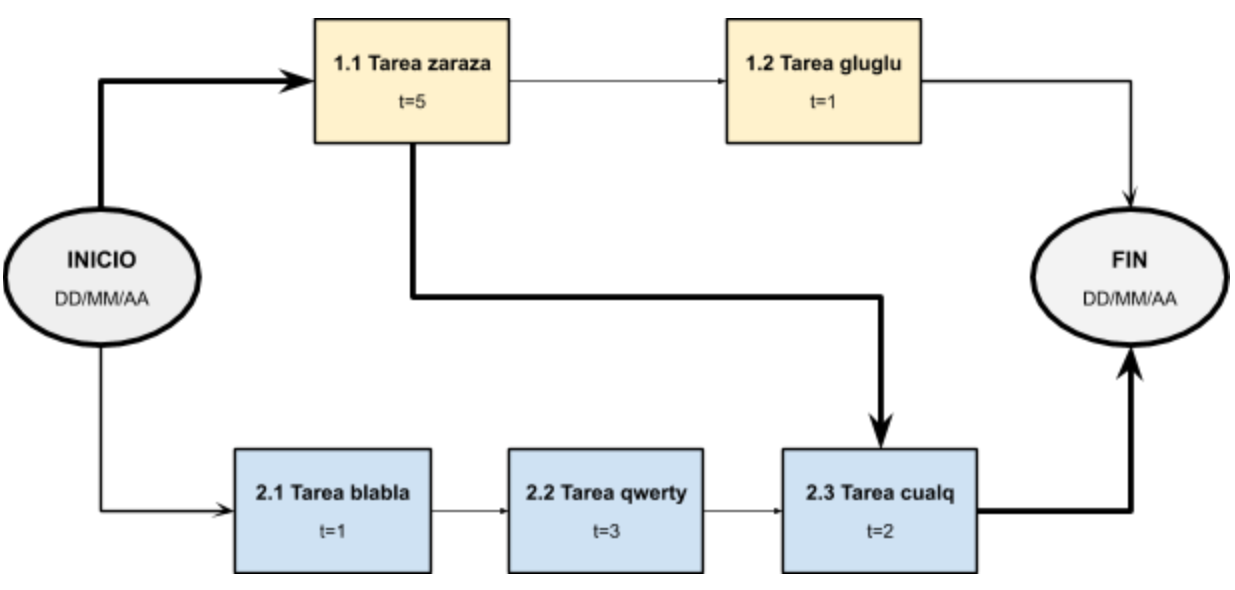
\includegraphics[width=.75\paperwidth]{./Figuras/AoN.png}
	\caption{Diagrama de \textit{Activity on Node}.}
	\label{fig:AoN}
\end{figure}

\section{11. Diagrama de Gantt}
En la figura \ref{fig:diagGantt} se presenta el diagrama de Gantt del proyecto.
Al solo disponer de una persona trabajando en el proyecto, las tareas no pueden paralelizarse y están dispuestas en cascada.
Cada día equivale a 4 horas de trabajo en el proyecto de acuerdo a lo descrito en la sección \ref{sec:supuestos}.

Además, las tareas opcionales no aparecen para no desvirtuar el diagrama estimado.
En caso de aplicarse estos objetivos secundarios, se enviará una actualizacion de dicho diagrama a los interesados.

\label{sec:gantt}
\begin{landscape}
	\begin{figure}[htpb]
		\centering
		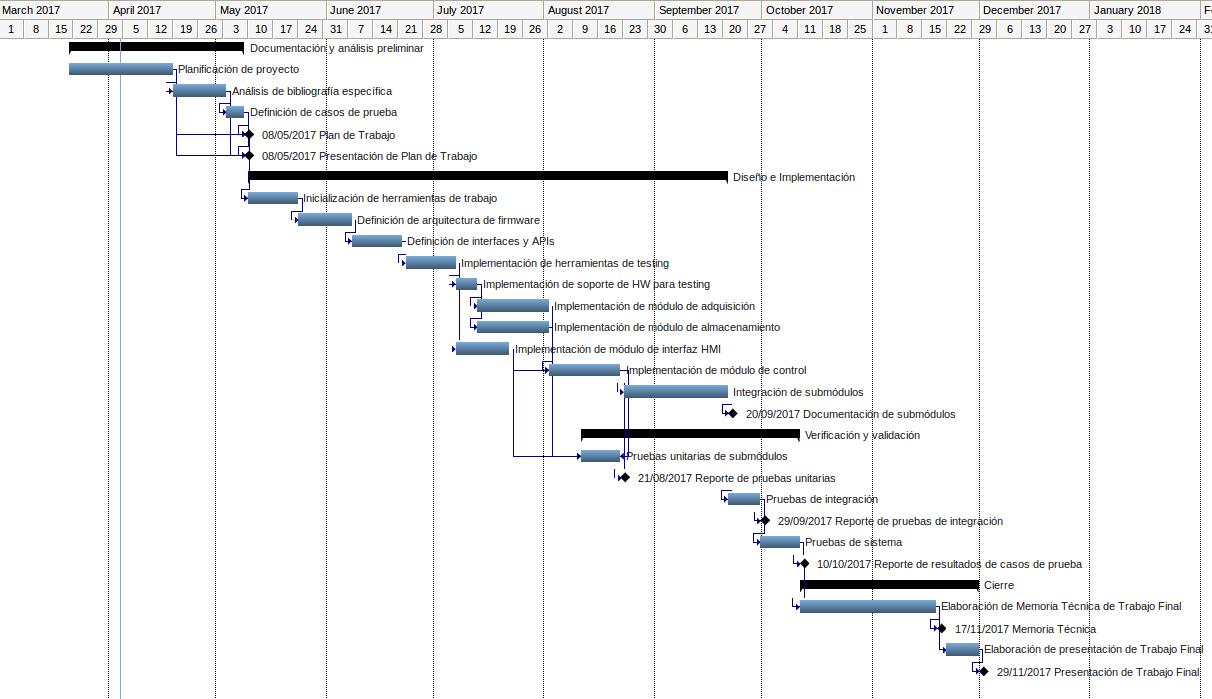
\includegraphics[height=.67\textheight]{./Figuras/Gantt-2.png}
		\caption{Diagrama de Gantt.}
		\label{fig:diagGantt}
	\end{figure}
\end{landscape}
\section{12. Presupuesto detallado del proyecto}
\label{sec:presupuesto}
Para el cómputo del valor de las horas de ingeniería se ha tomado como referencia el salario medio de un ingeniero software en España en el año 2023, cuyo valor es de \euro18,08 por hora.
Dicho valor se ha convertido a pesos argentinos bajo la tasa representativa del mercado del día 14/11/2023, una equivalencia de 380,96 pesos por euro.
Es decir, el valor del trabajo de ingeniería es de \$6.887,76 por hora.

También se utilizara el valor de conversión de euros a pesos para la estimación del coste del \textit{hardware} de trabajo.

\begin{table}[htpb]
	\centering
	\begin{tabularx}{\linewidth}{@{}|X|c|r|r|@{}}
		\hline
		\rowcolor[HTML]{C0C0C0}
		\multicolumn{4}{|c|}{\cellcolor[HTML]{C0C0C0}COSTOS DIRECTOS}       \\ \hline
		\rowcolor[HTML]{C0C0C0}
		Descripción                                                       &
		\multicolumn{1}{c|}{\cellcolor[HTML]{C0C0C0}Cantidad}             &
		\multicolumn{1}{c|}{\cellcolor[HTML]{C0C0C0}Valor unitario (ARS)} &
		\multicolumn{1}{c|}{\cellcolor[HTML]{C0C0C0}Valor total (ARS)}      \\ \hline
		Horas del Responsable (MVP)                                       &
		\multicolumn{1}{c|}{615}                                          &
		\multicolumn{1}{c|}{6.887,76}                                     &
		\multicolumn{1}{c|}{4.235.972,4}                                    \\ \hline
		Horas del Responsable (Opcional)                                  &
		\multicolumn{1}{c|}{80}                                           &
		\multicolumn{1}{c|}{6.887,76}                                     &
		\multicolumn{1}{c|}{551.020,8}                                      \\ \hline

		\multicolumn{3}{|c|}{SUBTOTAL}                                    &
		\multicolumn{1}{c|}{4.786.993,2}                                    \\ \hline
		\rowcolor[HTML]{C0C0C0}
		\multicolumn{4}{|c|}{\cellcolor[HTML]{C0C0C0}COSTOS INDIRECTOS}     \\ \hline
		\rowcolor[HTML]{C0C0C0}
		Descripción                                                       &
		\multicolumn{1}{c|}{\cellcolor[HTML]{C0C0C0}Cantidad}             &
		\multicolumn{1}{c|}{\cellcolor[HTML]{C0C0C0}Valor unitario (ARS)} &
		\multicolumn{1}{c|}{\cellcolor[HTML]{C0C0C0}Valor total (ARS)}      \\ \hline
		Hardware de trabajo                                               &
		\multicolumn{1}{c|}{1}                                            &
		\multicolumn{1}{c|}{609.536}                                      &
		\multicolumn{1}{c|}{609.536}                                        \\ \hline
		\multicolumn{3}{|c|}{SUBTOTAL}                                    &
		\multicolumn{1}{c|}{609.536}                                        \\ \hline
		\rowcolor[HTML]{C0C0C0}
		\multicolumn{3}{|c|}{TOTAL}                                       &
		\multicolumn{1}{c|}{5.396.529,2}                                    \\ \hline
	\end{tabularx}%
\end{table}

Se aclara de nuevo que \$551.020,8 del coste total se atribuyen a costes opcionales en caso de que se decida añadir funcionalidad adicional.

\section{13. Gestión de riesgos}
\label{sec:riesgos}
a) Se identificaron los siguientes riesgos para el proyecto:

Riesgo 1: No disponer de un modelo de tipo LLM preentrenado que sea adecuado para el proyecto.
\begin{itemize}
	\item Severidad (S): Se trata de un riesgo crítico ya que la ausencia de un modelo supondría la imposibilidad de realizar el proyecto. (10)
	\item Ocurrencia (O): La probabilidad de ocurrencia es baja porque hay múltiples opciones disponibles. (3)
\end{itemize}

Riesgo 2: \textit{Dataset} inadecuado para el \textit{fine-tuning} del modelo.
\begin{itemize}
	\item Severidad (S): Se trata de un riesgo severo ya que un entrenamiento inadecuado del modelo induciría a resultados insuficientes para el cliente. (8)
	\item Probabilidad de ocurrencia (O): La probabilidad de ocurrencia es media debido a varios factores.
	      Es necesario encontrar un \textit{dataset} lo suficientemente completo para empezar a procesarlo.
	      Además, no se dispone de conocimiento pleno a la hora de tratar adecuadamente con datos de esta naturaleza.
	      Se supone que se adquirirá experiencia en el desarrollo del curso de especialización. (5)
\end{itemize}

\pagebreak

Riesgo 3: Capacidad \textit{hardware} insuficiente.
\begin{itemize}
	\item Severidad (S): La severidad del riesgo es media porque provocaría retrasos en los tiempos de \textit{fine-tuning} y de predicción del modelo.
	      Esto podría provocar retrasos en el proyecto y un rendimiento insuficiente en los servicios. (5)
	\item Ocurrencia (O): La ocurrencia del riesgo es baja porque se cuenta con un equipo con una placa de video de buena calidad.
	      Además, es improbable que dicho equipo se dañe o se pierda. (3)
\end{itemize}

Riesgo 4: Retrasos en el proyecto.
\begin{itemize}
	\item Severidad (S): La severidad del riesgo es baja ya que el cliente es flexible en la extensión de los plazos. (3)
	\item Ocurrencia (O): La ocurrencia del riesgo es alta al tratarse de un proyecto que se inicia en mitad del curso de especialización.
	      Es posible que tanto la falta de experiencia como la carga de trabajo externa cause que no se disponga de todo el tiempo efectivo estimado para la realización del proyecto. (6)
\end{itemize}

Riesgo 5: Resultado final insuficiente.
\begin{itemize}
	\item Severidad (S): Se trata de un riesgo severo debido a que invalida gran parte de los requerimientos del proyecto. (8)
	\item Ocurrencia (O): Existe la posibilidad de que, a pesar de trabajar correctamente con el Modelo LLM y el \textit{dataset}, el resultado final no sea esperado por el cliente.
	      No existe una forma objetiva de ponderar el éxito del modelo. (4)
\end{itemize}
b) Tabla de gestión de riesgos:      (El RPN se calcula como RPN=SxO)

\begin{table}[htpb]
	\centering
	\begin{tabularx}{\linewidth}{@{}|X|c|c|c|c|c|c|@{}}
		\hline
		\rowcolor[HTML]{C0C0C0}
		Riesgo                                       & S  & O & RPN & S* & O* & RPN* \\ \hline
		1. Modelo LLM inadecuado.                    & 10 & 3 & 30  & 10 & 2  & 20   \\ \hline
		2. \textit{Dataset} inadecuado.              & 8  & 5 & 40  & 8  & 3  & 24   \\ \hline
		3. Capacidad \textit{hardware} insuficiente. & 5  & 3 & 15  & -  & -  & -    \\ \hline
		4. Retrasos en el proyecto.                  & 3  & 6 & 18  & -  & -  & -    \\ \hline
		5. Resultado final insuficiente.             & 8  & 4 & 32  & 6  & 3  & 18   \\ \hline
	\end{tabularx}%
\end{table}

Se van a adoptar medidas de mitigación para aquellos riesgos con valores RPN mayores a 30.

Nota: los valores marcados con (*) en la tabla corresponden luego de haber aplicado la mitigación.

c) Plan de mitigación de los riesgos que originalmente excedían el RPN máximo establecido:

Riesgo 1: No disponer de un modelo de tipo LLM preentrenado que sea adecuado para el proyecto.
El plan de mitigación consiste en dedicar tiempo y recursos adicionales en la búsqueda de modelos LLM.
Esto incluye considerar modelos en otros lenguajes de programación, siempre que se cuente con la experiencia necesaria.
También buscar documentación online o videos de divulgación de modelos de tipo LLM.
\begin{itemize}
	\item  Severidad (S*): La severidad no cambia ya que la integridad del proyecto depende de un modelo LLM compatible. (10)
	\item  Probabilidad de ocurrencia (O*): La probabilidad de ocurrencia es menor debido a los recursos adicionales empleados. (2)
\end{itemize}

Riesgo 2: \textit{Dataset} inadecuado para el \textit{fine-tuning} del modelo.
El plan de mitigación consiste en dedicar tiempo y recursos adicionales en la búsqueda y análisis de \textit{Dataset}.
La redacción del documento de análisis del dataset también ayuda a mitigar el riesgo.
\begin{itemize}
	\item  Severidad (S*): La severidad del riesgo no cambia. (8)
	\item  Probabilidad de ocurrencia (O*): La probabilidad de ocurrencia es menor debido a los recursos adicionales empleados. (3)
\end{itemize}

Riesgo 3: Resultado final insuficiente.
El plan de mitigación consiste en comunicarse con el cliente para acordar criterios de evaluación del \textit{output} de los servicios que sean razonables.
Siempre que sea posible se harán demostraciones del \textit{software} en las reuniones de seguimiento para detectar puntos de mejora antes de la finalización del proyecto.
Los test automáticos aportarán cobertura de código en la medida de lo posible.

\begin{itemize}
	\item  Severidad (S*): La severidad baja al conocer las expectativas del cliente. (6)
	\item  Probabilidad de ocurrencia (O*): La probabilidad de ocurrencia es menor debido a la demostración preeliminar de resultados. (3)
\end{itemize}


\section{14. Gestión de la calidad}
\label{sec:calidad}

\begin{itemize}
	\item Req \#1.2: El servidor debe contar con los procesos necesarios para entrenar la Inteligencia Artificial.
	      \begin{itemize}
		      \item Verificación: Consultar la base de datos para observar si los parámetros del módulo LLM se actualizan tras ejecutar el comando de entrenamiento.
		      \item Validación: En el manual de administrador se explicará el comando que entrena el módulo LLM.
		            Además, de ser requerido, se hará una demostración del rendimiento del modelo antes y después del \textit{fine-tuning}.
	      \end{itemize}

	\item Req \#1.3: Al ser desplegado, el servidor deberá iniciar el módulo LLM y utilizarlo en el procesamiento de peticiones entrantes.
	      \begin{itemize}
		      \item Verificación: Confirmar a través de inspección en el código y/o archivos de registro que el proceso de despliegue del servidor web incluye la inicialización del módulo LLM.
		      \item Validación: Se confirmará con el cliente que los servicios REST estén funcionando y su \textit{output} se ajuste a los criterios acordados.
	      \end{itemize}

	\item Req \#1.5: Los servicios REST deben aceptar entrada de texto en varios formatos: pdf, txt, word o texto plano en el cuerpo de la petición.
	      \begin{itemize}
		      \item Verificación: Se harán test automáticos que validen que la extracción de texto funcione correctamente.
		      \item Validación: En las peticiones REST se utilizarán archivos adjuntos como parametros de entrada y se confirmará una respuesta acorde.
	      \end{itemize}

	\item Req \#1.6: Los servicios REST devolverán la respuesta en formato simple HTML para su cómoda visualización en un navegador.
	      \begin{itemize}
		      \item Verificación: Inspección de código.
		      \item Validación: La respuesta de las peticiones REST se visualizarán en el navegador.
	      \end{itemize}

	\item Req \#2.2: El módulo LLM, si el texto de entrada es legible, debe aportar una respuesta con un detalle y profundidad razonables,
	      además de ser coherente con las instrucciones recibidas.
	      \begin{itemize}
		      \item Verificación: Se probará el comportamiento del módulo en varias pruebas a lo largo del desarrollo,
		            las cuales podrán incluirse en el documento de análisis del \textit{dataset} o en los informes de seguimiento del módulo LLM.
		      \item Validación: Se confirmará con el cliente que los resultados de las peticiones REST son satisfactorias.
	      \end{itemize}

	\item Req \#3.1: El proyecto contará con test automáticos que probarán el correcto funcionamiento de los módulos no relacionados con el modelo LLM.
	      \begin{itemize}
		      \item Verificación: Inspección de código.
		      \item Validación: Se describira brevemente al cliente la lista de test automáticos, mostrando su código si así se solicita.
	      \end{itemize}

	\item Req \#4.1: Se entregará un documento de administrador que explicará brevemente el sistema, qué comandos de ejecución tiene y los requisitos \textit{hardware} necesarios para su correcto funcionamiento.
	      \begin{itemize}
		      \item Verificación: Se seguirá el manual de administrador para comprobar que se despliega el proyecto sin problemas.
		      \item Validación: El cliente seguirá el manual de administrador para comprobar que se despliega el proyecto sin problemas.
	      \end{itemize}

	\item Req \#4.2: Se entregará un documento con un breve análisis de los resultados del módulo LLM que se hayan expuesto al cliente durante las reuniones de seguimiento.
	      \begin{itemize}
		      \item Verificación: Se asegurará que el contenido del documento sea adecuado.
		      \item Validación: El cliente confirmará que el documento está completo.
	      \end{itemize}

	\item Req \#5.1: Cualquier información del cliente que se utilice en el desarrollo del proyecto estará amparada por derechos de privacidad y propiedad intelectual.
	      \begin{itemize}
		      \item Verificación: Inspección de código. Los datos sensibles estarán ofuscados y/o encriptados.
		      \item Validación: Será imposible acceder a los datos sensibles a través del servidor web
	      \end{itemize}

\end{itemize}

\pagebreak

\section{15. Procesos de cierre}
\label{sec:cierre}
El proceso de cierre se realizará de la siguiente forma:

\begin{itemize}
	\item Reunion entre el responsable del proyecto y el cliente para analizar los resultados finales.
	      Se listarán conclusiones del proyecto, viabilidad para incluirlo en el producto Critial Match y posibles caminos de mejora.
	\item Reunion entre el responsable del proyecto y director de proyecto para analizar los resultados del proyecto de acuerdo con el plan definido.
	\item El responsable del proyecto escribirá un breve reporte, en forma de listado, de los aciertos y errores del proyecto.
	      También incluirá los desafíos inesperados a los que se enfrentó y las acciones tomadas para superarlos.
	\item Preparación de una presentación del trabajo y defensa pública.
	\item Al final de la defensa pública el responsable del proyecto dedicará unos minutos en realizar el acto de agradecimiento a todos los interesados, y en especial al equipo de trabajo y colaboradores.
	      Los agradecimientos también quedarán reflejados en la presentación y en la memoria del trabajo final.
	\item Al tratarse de un proyecto personal, no se prevee que haya financiación alguna de los gatos correspondientes del proyecto.
\end{itemize}
\end{document}
